%% Manuscript for the Journal of Network and Computer Applications (Elsevier), elsarticle class.
%% Build: latexmk -pdf jnca_main.tex   (from the paper/ directory)
\documentclass[preprint,12pt]{elsarticle}
% Searchable, copyable text for equations and symbols in the PDF text layer.
\input{glyphtounicode}
\pdfgentounicode=1
\usepackage{mmap}
\usepackage[T1]{fontenc}
% Packages and macros shared by the JNCA (elsarticle) and IEEE IoT-J (IEEEtran) versions.
\usepackage{amsmath,amssymb}
\usepackage{graphicx}
\usepackage{booktabs}
\usepackage{array}
\usepackage{tabularx}
\usepackage{adjustbox}
\usepackage{enumitem}
\usepackage{xcolor}
\usepackage{pifont}
\usepackage{tikz}
\usetikzlibrary{arrows.meta,positioning}
\usepackage{algorithm}
\usepackage{algpseudocode}
\usepackage{url}
\usepackage[hidelinks]{hyperref}

\newcommand{\cmark}{\ding{51}}            % provided
\newcommand{\xmark}{\ding{55}}            % not provided / not reported
\newcommand{\pmark}{$\sim$}              % partly
\renewcommand{\tabularxcolumn}[1]{p{#1}}
\makeatletter
\newcommand{\inputtab}[1]{\@@input #1 }   % \input that works inside a tabular (generated table rows)
\makeatother
\newcolumntype{L}[1]{>{\raggedright\arraybackslash}p{#1}}

\newenvironment{widetab}{\begin{table}[tp]}{\end{table}}   % single column: wide tables are ordinary tables
\journal{Journal of Network and Computer Applications}

\begin{document}
\begin{frontmatter}

\title{How close do WSN routers come to the lifetime bound? A reproducible benchmark of shortest-path, coordinated and learned multi-hop routing}

\author[inst1]{Shubham Mittal}
\author[inst1]{Aditya Periwal\corref{cor1}}
\ead{[corresponding author e-mail]}
\cortext[cor1]{Corresponding author.}
\affiliation[inst1]{organization={Netaji Subhas University of Technology}, city={New Delhi}, postcode={110078}, country={India}}

\begin{abstract}
Learning-based routers for wireless sensor networks are rarely compared with strong shortest-path baselines or with a lifetime bound, so their benefit is hard to judge. We benchmark multi-hop tree routing without aggregation against the Chang--Tassiulas fractional-flow bound, extended to an oracle for time-varying traffic, with every control bit charged: battery reports and route advertisements that encode every next hop. On 30 topologies under four traffic scenarios, battery-weighted Dijkstra reaches 85.2\% of the bound. Coordinating the routes chosen within a round adds about 4.5 points. Chang and Tassiulas's flow augmentation, run in within-round increments, reaches 89.9\%, and a sequential booked-load Dijkstra 89.7\%; at this operating point the two are indistinguishable (difference $-0.2$ points, 95\% CI $[-1.3, 0.8]$). An LP planner re-solved every round reaches 96.6\%, which shows that the bound is on average within 3.6\% of what a sequence of trees can achieve. On fresh topologies neither coordination mechanism dominates. Flow augmentation is ahead in small and clustered networks. Booked-load Dijkstra is ahead where traffic funnels hardest: with the sink at a corner it reaches 85.6\% against 79.3\%. Under lossy links with retransmissions and contention, coordination keeps its lifetime gain but lowers the delivery ratio. A reconstruction of a recent multi-agent reinforcement-learning router, with its reward and selection protocol corrected, collapses to direct transmission, although its own reward prefers Dijkstra routes eightfold; we report this as a reproducibility failure. When the sink can afford an LP per round, the planner is usually the better choice.

\end{abstract}

\begin{highlights}
\item Multi-hop WSN routers are scored against a fractional-flow lifetime bound.
\item Battery-weighted Dijkstra reaches 85\% of the bound with no training.
\item Within-round coordination adds about 4.5 points; two mechanisms tie.
\item An LP planner reaches 97\%, certifying the bound is nearly tight.
\item A corrected learned-router reconstruction collapses; we diagnose why.
\end{highlights}

\begin{keyword}
Wireless sensor networks \sep Network lifetime \sep Energy-efficient routing \sep Benchmarking \sep Maximum-lifetime linear program \sep Flow augmentation \sep Reproducibility
\end{keyword}

\end{frontmatter}

\section{Introduction}\label{sec:intro}

A wireless sensor network (WSN) forwards readings from battery-powered nodes to a sink over several hops. Every relayed bit costs energy, so the routing decides how long the network lasts. The time until the first node dies is a standard lifetime measure~\cite{chang2004maximum}.

Recent work proposes deep reinforcement learning for this routing problem~\cite{yang2025madii,younus2021sdwsn}. These methods are usually compared with clustering heuristics, metaheuristics or other learned methods. They are rarely compared with a battery-weighted shortest-path router, and rarely reported as a fraction of an achievable bound (Table~\ref{tab:practice}). Without both, it is hard to tell how much a new method contributes.

This paper is primarily a benchmark. We score routers against the Chang--Tassiulas fractional-flow bound~\cite{chang2004maximum}, extended to an oracle that knows future traffic, on held-out and fresh topologies. Every control bit the routers rely on is charged. We restrict the comparison to one family, multi-hop trees without aggregation, so that no protocol is evaluated outside the setting it was designed for. Within that family the results fall into clear levels:
\begin{itemize}[leftmargin=*]
  \item \textbf{Battery-weighted Dijkstra} reaches about 85\% of the bound, with no training.
  \item \textbf{Within-round coordination} adds about 4.5 points. Here the routes of one round account for each other, either through Chang and Tassiulas's flow augmentation run in small increments or through a sequential booked-load Dijkstra. The two mechanisms tie at the main operating point but not elsewhere: on fresh topologies flow augmentation is ahead in small and clustered networks, and booked-load Dijkstra where traffic funnels hardest towards the sink.
  \item \textbf{An LP planner} re-solved every round reaches about 97\%. This shows that the relaxation is close to what trees can achieve, and that the remaining gap belongs to the solver.
\end{itemize}

\paragraph{Contributions}
\begin{enumerate}[label=(C\arabic*), leftmargin=*]
  \item \textbf{A bound-normalised benchmark protocol.} It has charged control accounting, same-family baselines tuned on separate validation topologies, the topology as the statistical unit with bootstrap intervals, robustness on fresh topologies, and a released artifact.
  \item \textbf{A measured ranking with a tightness certificate.} At the main operating point the best realised router reaches 96.4\% of the bound on average, so the bound overstates the achievable lifetime by at most a few percent there and normalised scores can be read close to absolute. Under a corner sink with clustered nodes the certificate is much weaker (Section~\ref{sec:grid}).
  \item \textbf{Within-round coordination, in two complementary forms.} Flow augmentation (2004) and booked-load Dijkstra each add about 4.5 points over battery Dijkstra at the main operating point, where they tie. On fresh topologies they diverge: booked load gains up to 26 points over flow augmentation when the sink is at a corner of a clustered field, and flow augmentation gains about 4 points in small or clustered networks. Removing the battery term destroys either. Reporting load in quantised tiers costs nothing measurable, and it is unnecessary when the sink observes the traffic.
  \item \textbf{Realism and cost probes.} We report lossy links with ARQ and receiver contention, and the measured sink computation time from $n=50$ to $n=800$, which shows when avoiding the LP solver matters.
  \item \textbf{A reproducibility record.} We document the errors found in earlier versions of this study and corrected here (Appendix~\ref{app:corrections}). We also report a learned-router reconstruction that fails, with a diagnosis (Appendix~\ref{app:madii}).
\end{enumerate}

Section~\ref{sec:related} reviews related work. Section~\ref{sec:model} defines the model, its scope and its assumptions, Section~\ref{sec:methods} the routers and Section~\ref{sec:setup} the protocol. Section~\ref{sec:results} reports the results, Section~\ref{sec:discussion} discusses them together with the threats to validity, and Section~\ref{sec:conclusion} concludes.

\section{Related work}\label{sec:related}

\subsection{Energy models and clustering}
Heinzelman et al.~\cite{heinzelman2000leach} introduced the first-order radio model used by most WSN routing studies, including this one (Section~\ref{sec:radio}). Their LEACH protocol popularised clustering with rotating cluster heads. Later schemes elect cluster heads with fuzzy c-means or population metaheuristics. These protocols derive much of their benefit from in-network aggregation at cluster heads. This paper studies multi-hop tree routing \emph{without} aggregation, which is MADII's own setting~\cite{yang2025madii}. Cluster-based protocols are therefore outside its scope and are not used as comparators (Section~\ref{sec:scope}).

\subsection{Lifetime-optimal and energy-aware shortest-path routing}
Dijkstra's algorithm~\cite{dijkstra1959note} with radio energy as the link cost gives minimum-total-energy (MTE) routing, which exhausts the same relays first. Chang and Tassiulas~\cite{chang2004maximum} formulated maximum-lifetime routing as a linear program (LP) over link flows. They also proposed \emph{flow augmentation}: shortest-cost paths whose link costs combine energy per bit with the residual energy at both ends, recomputed as flow is added in small increments. They reported lifetimes close to the LP optimum and compared against MTE routing. Flow augmentation already coordinates successive routing decisions through the predicted residual energy, so it is the natural solver-free baseline for this study, and we evaluate it (Section~\ref{sec:fa}). Faster single-source shortest-path algorithms~\cite{duan2025sorting} compute the same paths and cannot change routing quality.

\subsection{Load-balanced routing trees}
Dai and Han~\cite{dai2003nodecentric} grow a tree from the sink by grafting heavy nodes onto light branches; as described in~\cite{shan2013lifetime}, their method ignores distance and energy. Shan et al.~\cite{shan2013lifetime} build a load-balanced \emph{shortest-path} tree, in which every sensor reaches the sink in its minimum hop count, by a layer-by-layer network-flow construction. With non-aggregated relaying they report about 85\% of an upper bound, and we implement their construction as a baseline. EBR-DA~\cite{mahdi2018ebrda} combines residual energy and buffer occupancy over a hop tree and is designed for an aggregation setting. Because our model has no buffers and no aggregation, we do not use it as a comparator. Combining energy and load in a route decision is therefore established, and so is building load-balanced trees.

\subsection{Learning-based routing}
MADII~\cite{yang2025madii} is a multi-agent deep Q-network with an Informer encoder~\cite{zhou2021informer}. Under centralised training and execution it selects every sensor's next hop. It is compared with clustering, metaheuristic and learned methods, but not with a shortest-path baseline or a lifetime bound. Younus et al.~\cite{younus2021sdwsn} train an RL agent in a software-defined WSN controller on a testbed and compare it with an RL-based WSN routing scheme. Tang et al.~\cite{tang2025twotier} apply multi-agent RL to topology optimisation in wireless mesh networks, targeting delay and power. A recent review~\cite{learning4routing2025} covers learning for routing more broadly, and recent comparison studies tabulate results from different datasets and units~\cite{icmcsi2026}. In network traffic classification, careful baselines have matched deep models~\cite{simplemodel2025}; this is a different task, but it is the same evaluation concern.

\subsection{Evaluation practice}
Table~\ref{tab:practice} records, for the closest studies, which evaluation elements each paper reports, as stated in its own text. Every criterion can be checked against the cited paper.

\begin{widetab}
\centering
\caption{Evaluation elements reported by the closest studies, as stated in each paper. \cmark: reported; \pmark: partly; \xmark: not reported.}\label{tab:practice}
\footnotesize
\setlength{\tabcolsep}{4pt}
\begin{adjustbox}{max width=\linewidth}
\begin{tabular}{@{}L{0.28\textwidth}*{6}{>{\centering\arraybackslash}p{0.095\textwidth}}@{}}
\toprule
Study & Shortest-path baseline & Lifetime bound & Time-varying traffic & Control energy charged & Statistical test & Code released\\
\midrule
Chang and Tassiulas~\cite{chang2004maximum} & \cmark & \cmark & \cmark & \xmark & \xmark & \xmark\\
Shan et al.~\cite{shan2013lifetime} & \xmark & \cmark & \xmark & \xmark & \xmark & \xmark\\
Mahdi et al., EBR-DA~\cite{mahdi2018ebrda} & \xmark & \xmark & \pmark & \xmark & \xmark & \xmark\\
Younus et al.~\cite{younus2021sdwsn} & \xmark & \xmark & \xmark & \cmark & \xmark & \xmark\\
Yang et al., MADII~\cite{yang2025madii} & \xmark & \xmark & \xmark & \pmark & \xmark & \xmark\\
This study & \cmark & \cmark & \cmark & \cmark & \cmark & \cmark\\
\bottomrule
\end{tabular}
\end{adjustbox}

\smallskip
\raggedright\footnotesize
Notes. Shan et al.\ compare with a node-centric tree and an upper bound. EBR-DA is evaluated on event-driven traffic against DRINA and InFRA. Younus et al.\ measure energy on a testbed, so control traffic is included physically. MADII charges a 0.1-kbit control packet but not the encoding of next-hop identifiers.
\end{widetab}

\section{System model, scope and assumptions}\label{sec:model}

\subsection{Network model and scope}\label{sec:scope}
There are $n$ static sensor nodes $V=\{1,\dots,n\}$ and one sink $s$. The main setting is MADII's published setting~\cite{yang2025madii}: $n=100$ nodes uniform in a $500\times500$~m field, with the sink at the centre and initial energy $E_0=0.5$~J. Time is divided into rounds. In round $t$ node $i$ generates $k_i(t)$ packets, each forwarded to the sink along the round's routing tree $p_t:V\to V\cup\{s\}$. Relays forward every bit they receive, as in MADII (``no data compression''). \textbf{Scope.} The study concerns multi-hop tree routing without in-network aggregation. Protocols whose benefit comes mainly from aggregation at cluster heads (LEACH-family clustering) or that are specified for an aggregation setting (EBR-DA) are therefore not used as comparators. Comparing them with full forwarding would test them outside the setting they were designed for.

\subsection{Radio energy model}\label{sec:radio}
Transmitting $k$ bits over distance $d$ and receiving $k$ bits cost
\begin{align}
E_{\mathrm{TX}}(k,d) &= \begin{cases} kE_{\mathrm{elec}} + k\,\varepsilon_{\mathrm{fs}}d^2, & d<d_0,\\ kE_{\mathrm{elec}} + k\,\varepsilon_{\mathrm{amp}}d^4, & d\ge d_0,\end{cases}\label{eq:tx}\\
E_{\mathrm{RX}}(k) &= kE_{\mathrm{elec}},\qquad d_0=\sqrt{\varepsilon_{\mathrm{fs}}/\varepsilon_{\mathrm{amp}}}\approx 87.7~\mathrm{m},\label{eq:rx}
\end{align}
with $E_{\mathrm{elec}}=50$~nJ/bit, $\varepsilon_{\mathrm{fs}}=10$~pJ/bit/m$^2$ and $\varepsilon_{\mathrm{amp}}=0.0013$~pJ/bit/m$^4$. We write $e_{\mathrm{tx}}(i,j)=E_{\mathrm{TX}}(1,d_{ij})$ and $e_{\mathrm{rx}}=E_{\mathrm{elec}}$.

\subsection{Packet layer and control accounting}\label{sec:packet}
Every bit any router relies on is charged, and the same charges apply to every router (Table~\ref{tab:params}):
\begin{enumerate}[label=(\roman*), leftmargin=*]
  \item \textbf{Data packets} carry 4{,}000 payload bits plus a 16-bit residual-battery report from the source, so $L=4{,}016$ bits travel on every hop. Every energy-aware router, the LP planner and MADII's state upload need the batteries at the sink. The report is therefore charged to all routers, not assumed free.
  \item \textbf{The route advertisement} must encode every node's next hop. It has a 100-bit header plus $n\lceil\log_2(n+1)\rceil$ bits, so $L_c=800$ bits at $n=100$, and every alive node pays $E_{\mathrm{RX}}(L_c)$ per round. An earlier version of this study charged only 100 bits, which cannot encode 100 identifiers; Appendix~\ref{app:corrections} lists this and the other corrections.
  \item \textbf{Traffic rates} used by the routers are counted by the sink from the packets it receives, which costs no extra bits. The tiered-load variant (Section~\ref{sec:lest}) instead reports load in 2-bit tiers on an extra byte per packet plus a $2n$-bit snapshot in the advertisement. It is charged accordingly and is an ablation only.
\end{enumerate}
A relay that cannot afford a transmission dies within the round, and the packets routed through it in that round are lost. A source whose path failed retries directly to the sink if its battery allows. No MAC frames, acknowledgements or retransmissions are modelled in the main bench; Section~\ref{sec:lossy} adds lossy links, ARQ and contention as a probe.

\begin{table}[t]
\centering
\caption{Network, radio and packet parameters.}\label{tab:params}
\footnotesize
\begin{adjustbox}{max width=\linewidth}
\begin{tabular}{@{}L{0.46\linewidth}L{0.48\linewidth}@{}}
\toprule
Parameter & Value\\
\midrule
Nodes, field, sink & 100, uniform in $500\times500$~m, centre\\
Initial energy $E_0$ & 0.5~J (trace bench 1.0 and 1.5~J)\\
Data packet $L$ & 4{,}000 payload + 16 battery bits\\
Advertisement $L_c$ & $100 + n\lceil\log_2(n+1)\rceil$ (800 at $n=100$)\\
Radio constants & $E_{\mathrm{elec}}$ 50~nJ/bit; $\varepsilon_{\mathrm{fs}}$ 10~pJ/bit/m$^2$; $\varepsilon_{\mathrm{amp}}$ 0.0013~pJ/bit/m$^4$\\
Aggregation & none (full forwarding)\\
Tiered-load ablation & +8 bits per packet; +$2n$ bits per advertisement\\
\bottomrule
\end{tabular}
\end{adjustbox}
\end{table}

\subsection{Traffic}\label{sec:traffic}
A day is 24 rounds, and every router receives 3 days of pre-deployment history. In the daily-surge scenario (R), the 20\% of nodes nearest a random point send Poisson traffic with mean 4 packets per round during a 6-round evening and 0.5 otherwise, and all other nodes have mean 1. In the constant scenario (N), every node sends one packet per round, which is MADII's static setting. Bursts (B) adds to R, each round with probability 0.05, a burst in which a random node sends five times its rate for 4 rounds. Pattern shift (D) moves the hotspot to a new set of nodes after two days; it is a robustness scenario that nothing is tuned on. As a second, trace-driven traffic generator we convert Intel Berkeley Lab readings~\cite{intellab2004} into packets by send-on-delta reporting (one heartbeat per hour plus a packet per 0.5~$^\circ$C or 100~lux change) on the 54-mote layout scaled to the $500$~m field. This yields traffic with a different autocorrelation structure. It is not measured radio traffic.

\subsection{Assumptions}\label{sec:assumptions}
\begin{enumerate}[label=\textbf{A\arabic*}, leftmargin=*]
  \item Static nodes with identical initial energy; no harvesting or battery replacement.
  \item One static, mains-powered sink; its computation is not charged to sensors (its cost is reported separately in Section~\ref{sec:scaling}).
  \item No obstacles; link cost depends only on distance through~\eqref{eq:tx}--\eqref{eq:rx}.
  \item Any node can reach any other node and the sink by power control.
  \item Main bench: ideal symmetric links and collision-free scheduling. Section~\ref{sec:lossy} relaxes this.
  \item Only transmission and reception consume energy; sensing, processing and idle listening are not modelled.
  \item No aggregation or compression.
  \item Round-based operation: the sink computes each round's tree before the round and broadcasts it in the advertisement.
  \item The sink knows every node's position.
  \item The sink learns residual batteries from the 16-bit reports of the previous round (charged, item~(i)).
  \item The sink learns traffic only from packets it has received; only the oracle bound sees future traffic.
  \item Nodes fail only by depletion; a relay that cannot afford its transmission dies within the round.
  \item Every router sees the same deployments and traffic, so all comparisons are paired.
\end{enumerate}

\subsection{Lifetime, the bound and its tightness}\label{sec:problem}
Let $F$ be the round in which the first node dies; $T=F-1$ completed death-free rounds is the lifetime. For example, if the first death happens during round 152, then $F=152$ and $T=151$. Let $f_{ij}\ge0$ be the total bits sent on link $i\to j$. For constant traffic, the fractional-flow ceiling~\cite{chang2004maximum} is
\begin{align}
&\max_{T,\,f\ge0}\; T \quad\text{subject to, for every } i\in V,\nonumber\\
&\textstyle\sum_j f_{ij}-\sum_k f_{ki} = L\,T,\label{eq:lp-flow}\\
&\textstyle\sum_j f_{ij}\,e_{\mathrm{tx}}(i,j)+\sum_k f_{ki}\,e_{\mathrm{rx}} + T\,E_{\mathrm{RX}}(L_c) \le E_0.\label{eq:lp-energy}
\end{align}
For time-varying traffic the right-hand side of~\eqref{eq:lp-flow} becomes $L\sum_{t<T}k_i(t)$, and $T^*$ is the largest $T$ for which the LP is feasible, found by bisection (an oracle that knows the future). Any sequence of routing trees that keeps all nodes alive for $T$ rounds gives a feasible flow, so $T\le T^*$. We report every router as $100\,T/T^*$. This is a percentage of a \emph{relaxation}, not of the best achievable sequence of trees. Its looseness is bounded empirically in Section~\ref{sec:tight}: on every case, the best realised router certifies that the achievable optimum lies between that router's lifetime and $T^*$.

\section{Routers}\label{sec:methods}

Every router computes the round's tree at the sink from the information in A8--A11 and broadcasts it in the advertisement. All routers in the main comparison build multi-hop trees with full forwarding.

\subsection{Shortest-path baselines}
\emph{Min-energy (MTE) Dijkstra} uses the link cost $e_{\mathrm{tx}}(i,j)+e_{\mathrm{rx}}$. \emph{Battery-weighted Dijkstra} multiplies it by $E_0/E_i$, the sender's inverse residual-battery fraction, and is recomputed every round:
\begin{equation}
w(i,j)=\bigl[e_{\mathrm{tx}}(i,j)+e_{\mathrm{rx}}\bigr]\,E_0/E_i.\label{eq:battery}
\end{equation}
In battery-weighted Dijkstra every node's path is computed independently, so within one round many nodes can select the same relay.

\subsection{Load-balanced shortest-path tree (Shan et al.)}
We implement the top-down construction of~\cite{shan2013lifetime}. Hop layers are built over a radio range $R$. Each new layer is attached to the previous one so that the largest branch load at the sink is minimised, using a bisection on the bound with a max-flow feasibility test and unit load per sensor, as in their model. Within the chosen branch a node takes the candidate parent with the fewest descendants. The tree is rebuilt when a node dies. We do not implement their distributed refinement step. $R$ is tuned on validation deployments ($R=110$~m).

\subsection{Flow augmentation (Chang and Tassiulas)}\label{sec:fa}
Flow augmentation~\cite{chang2004maximum} routes traffic in small increments on shortest-cost paths, updating the residual energy after each increment. We run it as a per-round planner. Over a horizon of $H$ rounds, each source's traffic is pushed in $K$ increments on shortest paths over the cost
\begin{equation}
c(i,j)=e_{\mathrm{tx}}(i,j)\,(E_0/E'_i)^x + e_{\mathrm{rx}}\,(E_0/E'_j)^x,\label{eq:fa}
\end{equation}
where $E'$ is the residual energy predicted after the increments already placed. Each node then forwards to the next hop that carries the largest share of its augmented flow. No solver is used. Validation chose $x=1$, $H=3$ and $K=30$ (Section~\ref{sec:setup}). Because $E'$ changes during the round's own increments, later increments avoid relays loaded by earlier ones. This is a form of within-round coordination.

\subsection{Booked-load Dijkstra}\label{sec:bld}
Booked-load Dijkstra coordinates one round's routes through \emph{load} instead of predicted energy. The sink processes nodes in increasing distance from the sink. For each node without a route it runs Dijkstra over
\begin{equation}
w(j,k)=\bigl[e_{\mathrm{tx}}(j,k)+e_{\mathrm{rx}}\bigr]\,\frac{E_0}{E_j}\Bigl(1+\kappa\,\frac{A_j}{\bar r}\Bigr),\label{eq:bld}
\end{equation}
where $A_j$ is the traffic already booked through node $j$ in this round's construction and $\bar r$ is the mean node rate. It then fixes the path and books the source's rate on every node of it. A node that already received a route as a relay keeps its next hop, and its own rate is booked along that fixed path when its turn comes. Rates $r_i$ are the sink's count of packets received from $i$ over the last 24 rounds, so no extra bits are needed. With $\kappa=0$ the method is battery-weighted Dijkstra. Validation chose $\kappa=0.5$, and Section~\ref{sec:kappa} sweeps $\kappa$ on fresh deployments. Algorithm~\ref{alg:bld} gives one round.

\begin{algorithm}[t]
\caption{Booked-load Dijkstra: one round at the sink}\label{alg:bld}
\small
\begin{algorithmic}[1]
\Require alive nodes $V$, batteries $E_j$, observed rates $r_j$, link energies, weight $\kappa$
\Ensure parent function $p$
\State $A_j\gets0$, $p(j)\gets\bot$ for all $j$; $\bar r\gets$ mean of $r_j$
\For{$i\in V$ in increasing distance to the sink}
  \If{$p(i)\ne\bot$}
    \State $u\gets i$; \textbf{while} $u\ne s$: $A_u\gets A_u+r_i$, $u\gets p(u)$ \Comment{book own traffic}
    \State \textbf{continue}
  \EndIf
  \State arc weights from~\eqref{eq:bld}; for $j$ with $p(j)\ne\bot$ keep only $j\to p(j)$
  \State $P\gets$ Dijkstra least-cost path from $i$ to $s$
  \For{each $u$ on $P$ except $s$}
    \If{$p(u)=\bot$} $p(u)\gets$ successor of $u$ on $P$ \EndIf
    \State $A_u\gets A_u+r_i$
  \EndFor
\EndFor
\State \Return $p$
\end{algorithmic}
\end{algorithm}

\subsection{Ablations of booked-load Dijkstra}\label{sec:lest}
\emph{Load only} removes the battery factor from~\eqref{eq:bld}. \emph{Tiered load} replaces the sink-observed rates with load reported in four tiers (boundaries 0.15, 0.40, 0.75 of twice the largest historical rate, with a 0.05 hysteresis band). This is the Lightweight State Table design of our earlier work, and it is charged as in Section~\ref{sec:packet}. In a centralised sink the observed rates are free, so the tiered variant cannot gain. It is reported to quantify what quantised sharing would cost in a setting where nodes, not the sink, need the load.

\subsection{Upper reference: LP planner}\label{sec:lp-planner}
The sink re-solves the LP~\eqref{eq:lp-flow}--\eqref{eq:lp-energy} every round from the current batteries. Each node generates its observed mean rate, and a small total-energy term $\mu=10^{-3}$ favours low-energy flows. Every node then sends to the next hop with the largest LP share; credits are reset at each solve, so this is a deterministic rounding of the flow, not proportional rotation. It uses the same information as the routers above and is the strongest realisable router we found. It needs an LP solver at the sink.

\begin{widetab}
\centering
\caption{What each router needs ($n=100$). Times are single-thread wall-clock per round, mean over the main bench.}\label{tab:characteristics}
\footnotesize
\begin{adjustbox}{max width=\linewidth}
\begin{tabular}{@{}L{0.25\textwidth}L{0.24\textwidth}L{0.22\textwidth}L{0.12\textwidth}r@{}}
\toprule
Router & Information at the sink & Work per round & Extra bits & ms/round\\
\midrule
\inputtab{body/rev_char.tex}
\bottomrule
\end{tabular}
\end{adjustbox}
\end{widetab}

\section{Evaluation protocol}\label{sec:setup}

\paragraph{Splits} Test topologies use seeds 0--29, each with all four scenarios (traffic seed = topology seed + 1000). Every free setting was chosen on separate validation topologies 500--511 (scenarios R, N, B) before any test run:
\begin{itemize}[leftmargin=*]
  \item flow augmentation: $x\in\{0.5,1,2,5,20,50\}$, $H\in\{1,2,3,6,24,96\}$, $K\in\{5,10,30\}$;
  \item Shan's range: $R\in\{90,110,125,150,200\}$~m;
  \item booked-load: $\kappa\in\{0.5,1,2\}$.
\end{itemize}
The robustness grid (Section~\ref{sec:grid}) and the $\kappa$ sweep (Section~\ref{sec:kappa}) use \emph{fresh} topologies 2000--2029 that were never used for tuning or testing. Test runs were executed once with the settings fixed in the released code.

\paragraph{Statistical unit} A topology's primary score for a router is the mean of its R, N and B scores; D is reported separately. The four scenarios share a topology, so the 120 topology--scenario cases are not independent, and win/tie/loss counts over them are descriptive only. Paired comparisons use the 30 topology means. We lead with the mean paired difference and its 95\% bootstrap confidence interval over topologies (20{,}000 resamples)~\cite{efron1993bootstrap}, and the matched-pairs rank-biserial correlation $r$~\cite{kerby2014}. Two-sided Wilcoxon signed-rank $p$-values~\cite{wilcoxon1945,demsar2006} with Holm adjustment~\cite{holm1979} over the eight comparisons of Table~\ref{tab:stats} are reported for completeness. The routers are deterministic, so a small $p$ only states that one router is consistently ahead on this topology generator. The effect size and the interval carry the evidence.

\section{Results}\label{sec:results}

\subsection{Main benchmark}\label{sec:main}
Table~\ref{tab:main} reports every router on the 30 test topologies.
\begin{itemize}[leftmargin=*]
  \item \textbf{Battery-weighted Dijkstra} reaches 85.2\% of the bound on the R/N/B mean.
  \item \textbf{Within-round coordination} adds about 4.5 points. Flow augmentation in within-round increments reaches 89.9\% and booked-load Dijkstra 89.7\%; both beat battery Dijkstra on all 30 topologies.
  \item \textbf{The LP planner} reaches 96.6\% with a worst topology of 93.9\%.
  \item \textbf{Shan et al.'s tree and MTE} stay near 25\%. In this radio model, a minimum-hop tree forces long, energy-expensive hops ($d^4$ beyond 87.7~m), and its balance is built once. MTE drains the same relays first.
\end{itemize}
Fig.~\ref{fig:paired} shows the topology-level pairs: booked-load Dijkstra is above battery Dijkstra everywhere and scattered on both sides of flow augmentation.

\begin{widetab}
\centering
\caption{Lifetime as a percentage of the fractional-flow bound (30 test topologies). R: daily surge; N: constant (MADII's static setting); B: bursts; D: pattern shift, not tuned on. $S$ is the R/N/B mean; Worst is the lowest topology mean. The last column is the paired difference to battery-weighted Dijkstra on topology means, with a 95\% bootstrap CI.}\label{tab:main}
\footnotesize
\setlength{\tabcolsep}{4pt}
\begin{adjustbox}{max width=\linewidth}
\begin{tabular}{@{}L{0.27\textwidth}rrrrrrr@{}}
\toprule
Router & R & N & B & $S$ & Worst & D & vs battery Dijkstra\\
\midrule
\inputtab{body/rev_main.tex}
\bottomrule
\end{tabular}
\end{adjustbox}
\end{widetab}

\begin{figure}[t]
\centering
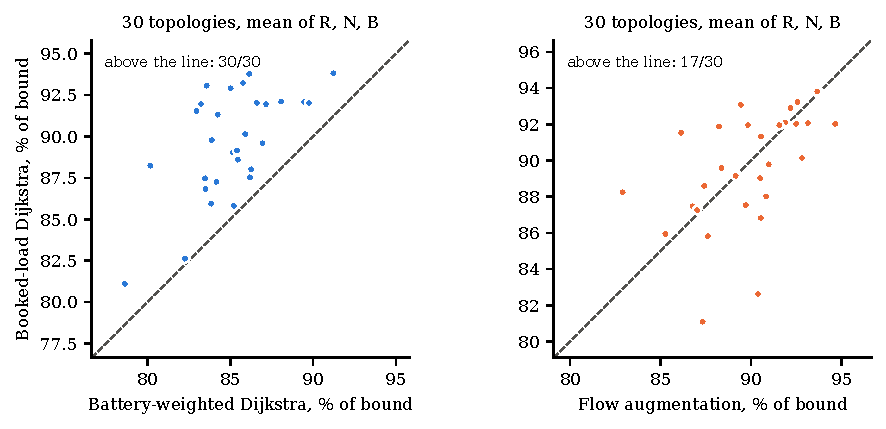
\includegraphics[width=\linewidth]{figs/rev_paired.pdf}
\caption{Topology means (R, N, B) of booked-load Dijkstra against battery-weighted Dijkstra (left) and against flow augmentation (right). Points above the dashed line favour booked-load Dijkstra.}\label{fig:paired}
\end{figure}

\subsection{Paired comparisons}\label{sec:stats}
Table~\ref{tab:stats} gives the eight planned comparisons on topology means. The difference between booked-load Dijkstra and flow augmentation is $-0.2$ points with a 95\% interval of $[-1.3, 0.8]$, so the two are indistinguishable. Over the 120 topology--scenario cases, which are descriptive only, booked-load Dijkstra wins 110, ties 7 and loses 3 against battery Dijkstra; flow augmentation wins 115, ties 4 and loses 1.

\begin{widetab}
\centering
\caption{Planned paired comparisons on topology means ($n=30$). Mean difference in points with a 95\% bootstrap CI, topology wins/ties/losses, rank-biserial $r$, and Holm-adjusted Wilcoxon $p$ over these eight comparisons.}\label{tab:stats}
\footnotesize
\setlength{\tabcolsep}{4pt}
\begin{adjustbox}{max width=\linewidth}
\begin{tabular}{@{}L{0.43\textwidth}rrrr@{}}
\toprule
Comparison & Difference [95\% CI] & W/T/L & $r$ & $p_{\mathrm{Holm}}$\\
\midrule
\inputtab{body/rev_stats.tex}
\bottomrule
\end{tabular}
\end{adjustbox}
\end{widetab}

\subsection{How tight is the bound?}\label{sec:tight}
The bound is a relaxation, so a percentage of it is only meaningful if it is close to what trees can achieve. On every topology--scenario case, the best realised router gives a lower bound on the achievable lifetime. Averaged over the 120 cases that router reaches 96.4\% of the bound, and its lowest case is 89.1\%. The achievable optimum therefore lies within 3.6 points of the bound on average, and within 10.9 points in the worst case. A score of 85\% therefore means at least $85/96.4\approx 88\%$ of what the best known tree sequence achieved, and at most 85\% of the true optimum.

\subsection{Ablations and the load weight}\label{sec:kappa}
Removing the battery term from booked-load Dijkstra lowers it to 40.7\% ($-49.0$ points): load spreading alone keeps relaying through nodes that are running out. Reporting load in four quantised tiers instead of the sink's observed counts changes the score by $-0.2$ points (CI $[-0.8, 0.3]$). This is not distinguishable from zero, but the tiers buy nothing either, because a centralised sink already observes the traffic for free. On fresh topologies (Table~\ref{tab:kappa}), \inputtab{body/rev_kappa_text.tex}

\begin{table}[t]
\centering
\caption{Load weight $\kappa$ of booked-load Dijkstra on 30 fresh topologies (seeds 2000--2029), R and N scenarios. $\kappa=0$ is battery-weighted Dijkstra.}\label{tab:kappa}
\footnotesize
\setlength{\tabcolsep}{3pt}
\begin{adjustbox}{max width=\linewidth}
\begin{tabular}{@{}rrrrl@{}}
\toprule
$\kappa$ & R & N & Mean & vs $\kappa=0$ [95\% CI]\\
\midrule
\inputtab{body/rev_kappa.tex}
\bottomrule
\end{tabular}
\end{adjustbox}
\end{table}

\subsection{Robustness on fresh topologies}\label{sec:grid}
Table~\ref{tab:grid} and Fig.~\ref{fig:grid} repeat the comparison on fresh topologies under five changed conditions: smaller and larger networks in the same field, the sink at a corner, clustered deployments, and both changes together. \inputtab{body/rev_grid_text.tex}

\begin{widetab}
\centering
\caption{Robustness on 30 fresh topologies per condition (seeds 2000--2029), mean of R and N, \% of the bound. The LP planner is omitted at $n=200$ (its per-round solve made the full grid impractical; see Table~\ref{tab:scaling}). The last two columns are paired differences on topology means with 95\% CIs.}\label{tab:grid}
\footnotesize
\setlength{\tabcolsep}{3pt}
\begin{adjustbox}{max width=\linewidth}
\begin{tabular}{@{}L{0.17\textwidth}rrrrrrrr@{}}
\toprule
Condition & MTE & Shan & Battery & FA & Booked & LP & Booked $-$ Battery & Booked $-$ FA\\
\midrule
\inputtab{body/rev_grid.tex}
\bottomrule
\end{tabular}
\end{adjustbox}
\end{widetab}

\begin{figure}[t]
\centering
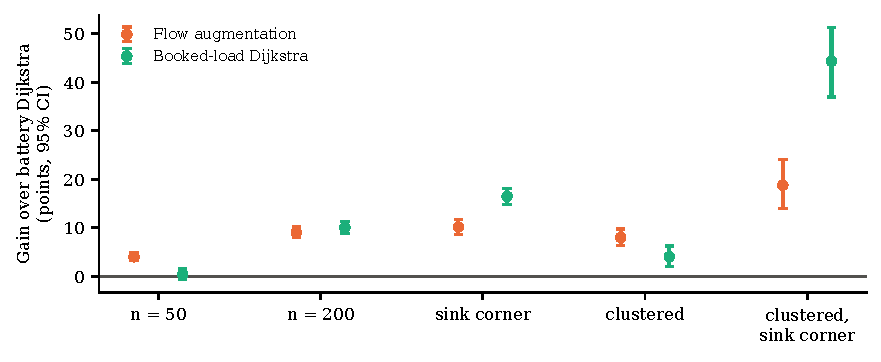
\includegraphics[width=\linewidth]{figs/rev_grid.pdf}
\caption{Gain over battery-weighted Dijkstra on fresh topologies, with 95\% bootstrap intervals over topologies.}\label{fig:grid}
\end{figure}

\subsection{Lossy links and contention}\label{sec:lossy}
Within-round coordination spreads traffic over more relays, which changes contention. We therefore probe the ideal-channel assumption once. Each link has a per-attempt reception rate that falls logistically with distance (50\% at 120~m, width 15~m) under static log-normal shadowing ($\sigma=0.1$), a common shape for the transitional region of low-power links~\cite{zuniga2004transitional}. ARQ allows up to four attempts, and both sender and receiver pay for every attempt. Routers and the bound use the expected energy per delivered bit, an ETX-style metric~\cite{decouto2003etx}. In the contention variant, each receiver's reception rate is further multiplied by $\exp(-I_j/C)$, where $I_j$ is the number of bits sent within 100~m of the receiver in that round and $C=2$~Mbit. No router knows this term. \inputtab{body/rev_lossy_text.tex}

\begin{widetab}
\centering
\caption{Lossy-link probe (test topologies 0--29, R and N). Lifetime as \% of the loss-aware bound, paired difference to battery Dijkstra, delivery ratio over the lifetime, and payload delivered before the first death.}\label{tab:lossy}
\footnotesize
\setlength{\tabcolsep}{3pt}
\begin{adjustbox}{max width=\linewidth}
\begin{tabular}{@{}llrlrr@{}}
\toprule
Link model & Router & Lifetime & vs battery [95\% CI] & Delivery (\%) & Mbit delivered\\
\midrule
\inputtab{body/rev_lossy.tex}
\bottomrule
\end{tabular}
\end{adjustbox}
\end{widetab}

\subsection{Trace-driven traffic (Intel Lab)}\label{sec:trace}
Table~\ref{tab:trace} uses the Intel-derived traffic generator on 27 overlapping start windows. The windows share one layout and overlap in time, and some runs outlast the trace and are censored (scored on their observed rounds). We therefore report the results descriptively, as a second traffic generator with a different autocorrelation structure, and draw no inferential claim from them. \inputtab{body/rev_trace_text.tex}

\begin{widetab}
\centering
\caption{Trace-driven traffic from Intel Lab readings (27 overlapping windows, scaled 54-mote layout). Mean and worst \% of the horizon-truncated bound; Cens.\ counts runs that outlast the trace. Descriptive only.}\label{tab:trace}
\footnotesize
\setlength{\tabcolsep}{4pt}
\begin{adjustbox}{max width=\linewidth}
\begin{tabular}{@{}L{0.30\textwidth}rrrrrr@{}}
\toprule
& \multicolumn{3}{c}{$E_0=1.0$~J} & \multicolumn{3}{c}{$E_0=1.5$~J}\\
\cmidrule(lr){2-4}\cmidrule(l){5-7}
Router & Mean & Worst & Cens. & Mean & Worst & Cens.\\
\midrule
\inputtab{body/rev_trace.tex}
\bottomrule
\end{tabular}
\end{adjustbox}
\end{widetab}

\subsection{Computation at the sink}\label{sec:scaling}
Table~\ref{tab:scaling} gives the single-thread time of one routing decision as the network grows at constant density, and the time of one sparse LP solve of the lifetime problem, which the planner repeats every round. \inputtab{body/rev_scaling_text.tex}

\begin{table}[t]
\centering
\caption{Single-thread wall-clock time of one routing decision (ms) and of one sparse LP solve (s), constant node density.}\label{tab:scaling}
\footnotesize
\setlength{\tabcolsep}{4pt}
\begin{adjustbox}{max width=\linewidth}
\begin{tabular}{@{}rrrrr@{}}
\toprule
$n$ & Battery (ms) & FA (ms) & Booked (ms) & LP solve (s)\\
\midrule
\inputtab{body/rev_scaling.tex}
\bottomrule
\end{tabular}
\end{adjustbox}
\end{table}

\section{Discussion}\label{sec:discussion}

\paragraph{What the bound shows} The ranking is clear. Battery weighting alone moves MTE from 25\% to 85\% of the bound. Within-round coordination adds about 4.5 points, and per-round LP planning another 7. Since the best realised router reaches 96.4\% of the bound, the remaining distance to the bound is mostly what the solver buys, not slack in the relaxation.

\paragraph{When does avoiding the solver matter?} In the modelled system the sink is mains-powered and its computation is free (A2), and Table~\ref{tab:scaling} shows that an LP solve fits within an hour-long round even at $n=800$. Within this model the rational choice is therefore the LP planner, and we recommend it. Solver-free coordination is worth having only outside the model: on an embedded gateway without an LP solver, with short rounds, for much larger networks, or as the basis of a distributed implementation in which nodes compute routes themselves. We do not evaluate a distributed implementation. The coordinated routers are therefore offered as the best option \emph{when the solver is not available}, not as an advance over it.

\paragraph{Two forms of within-round coordination} Both coordinated routers make later routing decisions of a round see the consequences of earlier ones. Flow augmentation does this through the residual energy predicted after each increment, booked-load Dijkstra through the traffic already booked on each relay. Both are successive-shortest-path constructions with incremental pricing, the idea of flow augmentation~\cite{chang2004maximum} applied within a round. They tie at the main operating point but diverge elsewhere (Table~\ref{tab:grid}). A plausible explanation follows. Booked load prices congestion directly, in proportion to the traffic routed through a relay. That matters most where traffic funnels hardest, as with a corner sink, where all traffic converges on a few relays. Energy prediction reacts only through the energy those relays would spend within a short horizon, which is a small fraction of their battery. In small or clustered networks, where funnelling is weaker, the energy-based price is the better guide. The mechanism therefore matters, and the choice depends on the topology. Flow augmentation is the faster default (2.5 times faster at $n=100$); booked-load Dijkstra is preferable where a single sink collects from a wide field. Neither works without the battery term.

\paragraph{Why Shan's tree and EBR-style designs score low here} Shan et al.'s construction is optimal for its own objective: a minimum-hop tree with balanced descendant counts under uniform energy. In a radio model whose transmit energy grows with $d^2$ to $d^4$ and with full power control (A4), the minimum-hop constraint forces long hops, and a tree built once cannot follow residual batteries. Its low score therefore reflects a mismatch between the protocol's assumptions and this model, not a defect of the protocol. The same reasoning is why aggregation-based protocols are out of scope (Section~\ref{sec:scope}).

\paragraph{Learned routing} Our corrected reconstruction of a recent multi-agent DRL router did not learn a non-trivial policy (Appendix~\ref{app:madii}). The corrected reward prefers Dijkstra-like routes about eightfold, so the failure is one of learning, not of the objective. This says nothing definitive about MADII as published: a comparison with the authors' implementation is needed before any claim about learned routing in general.

\subsection{Threats to validity}\label{sec:threats}
\begin{itemize}[leftmargin=*]
  \item \textbf{Radio and MAC.} The main bench assumes ideal links and collision-free scheduling. The lossy-link probe uses an expected-value ARQ model and a simple contention term, not a packet-level CSMA simulation. It shows that the lifetime gain survives but costs delivery; a packet-level MAC study could change the magnitudes.
  \item \textbf{Accounting.} Battery reports (16 bits) and the encoded advertisement are charged. Synchronisation, neighbour discovery and the reliability of the advertisement itself are not.
  \item \textbf{Traffic.} The synthetic generators are ours. The Intel-derived traffic is a trace-driven generator on a scaled layout, not measured radio traffic, and its overlapping, censored windows support no inferential claim.
  \item \textbf{Generality.} Fresh topologies cover $n\in\{50,100,200\}$, two sink positions and two layouts in one field size. Other densities, heterogeneous batteries and mobility are untested.
  \item \textbf{Baselines.} Flow augmentation is used as a per-round planner with tuned exponent and horizon. Shan's tree omits its distributed refinement step. The learned router is a reconstruction.
  \item \textbf{Reuse of test topologies.} The main test topologies 0--29 were also used by earlier versions of this study. Every setting was fixed on validation topologies, and the robustness grid and $\kappa$ sweep use topologies never seen before.
\end{itemize}

\section{Conclusion}\label{sec:conclusion}

Measured against the fractional-flow bound, multi-hop tree routing without aggregation falls into three levels:
\begin{itemize}[leftmargin=*]
  \item battery-weighted Dijkstra reaches about 85\%;
  \item within-round coordination reaches about 90\%, through flow augmentation run in increments or through booked-load Dijkstra, which tie at the main operating point;
  \item an LP planner re-solved every round reaches about 97\%.
\end{itemize}
At the main operating point the best realised router comes within a few percent of the bound, so there the bound is a meaningful yardstick. Removing the battery term destroys either coordinated router, and tiered load reporting is unnecessary at a centralised sink. On fresh topologies the two coordination mechanisms diverge: booked load is clearly better where traffic funnels towards a corner sink, flow augmentation in small or clustered networks. A reconstruction of a recent learned router failed to learn a non-trivial policy even though its own reward strongly prefers one. We report that as a limit of our reconstruction, together with the corrections made to earlier versions of this study.

For practice, a sink that can afford an LP per round should usually use the planner; the one exception in our grid was a corner sink over a clustered field, where booked-load Dijkstra did better. A sink that cannot, because it is embedded or the network is large, should use within-round coordination: the 2004 flow augmentation by default, and booked-load Dijkstra when the sink sits at the edge of a large or clustered field. Future work should evaluate the authors' implementation of learned routers, distributed coordination with an explicit control protocol, and packet-level MAC simulation.

\providecommand{\appendices}{\appendix}
\appendices
\section{Corrections relative to earlier versions}\label{app:corrections}
Reviewing the code before this revision found the following errors. All results in this paper come from the corrected code, and the released repository records each fix with a regression test.
\begin{enumerate}[label=(\alph*), leftmargin=*]
  \item \textbf{Booking omission.} In the sequential construction, a node that had already received its route as a relay on an earlier path never booked its own traffic. Its own rate is now booked along its fixed path (Algorithm~\ref{alg:bld}, lines 3--5). A test checks that booked loads equal the subtree sums of the final tree. With this fix the earlier ``90.5\%, 118 of 120 wins'' became the smaller gain reported here.
  \item \textbf{Cumulative energy in the learned router's reward.} The energy term of MADII's reward (its Eq.~15 defines $E_{\mathrm{start}}$ at the start of the round) was computed since deployment. It is now per round.
  \item \textbf{Checkpoint selection on test topologies.} The learned router's checkpoints were selected on topologies 0--4, which belong to the test set. Selection now uses topologies 500--504.
  \item \textbf{Control accounting.} The route advertisement was charged 100 bits, which cannot encode $n$ next-hop identifiers. Residual-battery reports were assumed free, while load reports were charged. Both are now charged as in Section~\ref{sec:packet}, identically for every router.
  \item \textbf{Metrics.} The hop count included one extra hop, and the tiered-load header was counted as delivered data. Both are fixed.
  \item \textbf{Statistical unit.} Earlier tests treated 120 topology--scenario cases as independent. They now use 30 topology means.
\end{enumerate}

\section{Learned-router reconstruction: a reproducibility failure}\label{app:madii}
No code for MADII~\cite{yang2025madii} is available. Our reconstruction uses an Informer-style encoder ($d_{\mathrm{model}}=128$, two layers, four heads) with a dot-product next-hop head, not the full published encoder--decoder. It is trained for 1{,}000 episodes: 300 with replay transitions from FCM, HBA and POA experts, then 700 with $\varepsilon$ decaying from 0.1 to 0.01. It uses Adam ($10^{-4}$), batch 64, replay 10{,}000, discount 0.99, Double DQN~\cite{vanhasselt2016double}, and checkpoint selection on validation topologies only. Three training seeds were run. \inputtab{body/rev_madii.tex}

This outcome characterises our reconstruction, not MADII: the published paper reports 19 rounds to first death in its own experiments. We therefore do not include the reconstruction in the main comparison.

% Back matter for the Elsevier (JNCA) version. AUTHORS: confirm every item before submission.

\section*{CRediT authorship contribution statement}
\textbf{Shubham Mittal:} [roles]. \textbf{Aditya Periwal:} [roles].

\section*{Declaration of competing interest}
The authors declare that they have no known competing financial interests or personal relationships that could have appeared to influence the work reported in this paper.

\section*{Data availability}
The simulator, every router, all raw result files, the corrected learned-router checkpoints and the scripts that regenerate every table and figure are available at \url{https://github.com/ShubhamMittal-17/madii-repro} (branch \texttt{aditya/wsn-routing}, directory \texttt{revision/}). The Intel Berkeley Lab data are publicly available~\cite{intellab2004}.

\section*{Declaration of generative AI and AI-assisted technologies in the manuscript preparation process}
% Elsevier and IEEE require every tool that was used to be named. Both tools below were used in this project.
During the preparation of this work the authors used Claude (Anthropic) and ChatGPT/Codex (OpenAI) to assist with code development, code review and debugging, experiment automation, statistical analysis and manuscript drafting and revision. After using these tools, the authors reviewed and edited the content as needed and take full responsibility for the content of the published article.

\section*{Acknowledgements}
[Funding statement, or: This research did not receive any specific grant from funding agencies in the public, commercial, or not-for-profit sectors.]


\bibliographystyle{elsarticle-num}
\bibliography{refs}

\end{document}
